\section{Модель плотности Земли}
\label{sec:prem}
В качестве модели плотности используется модель PREM~\cite{dziewonskiPREM1981}, которая предполагает сферическую симметрию и описывает плотность, давление и другие параметры как функции радиуса. Плотность в модели представлена на рис.~\ref{PREM}.

\begin{figure}[!h]
\centering
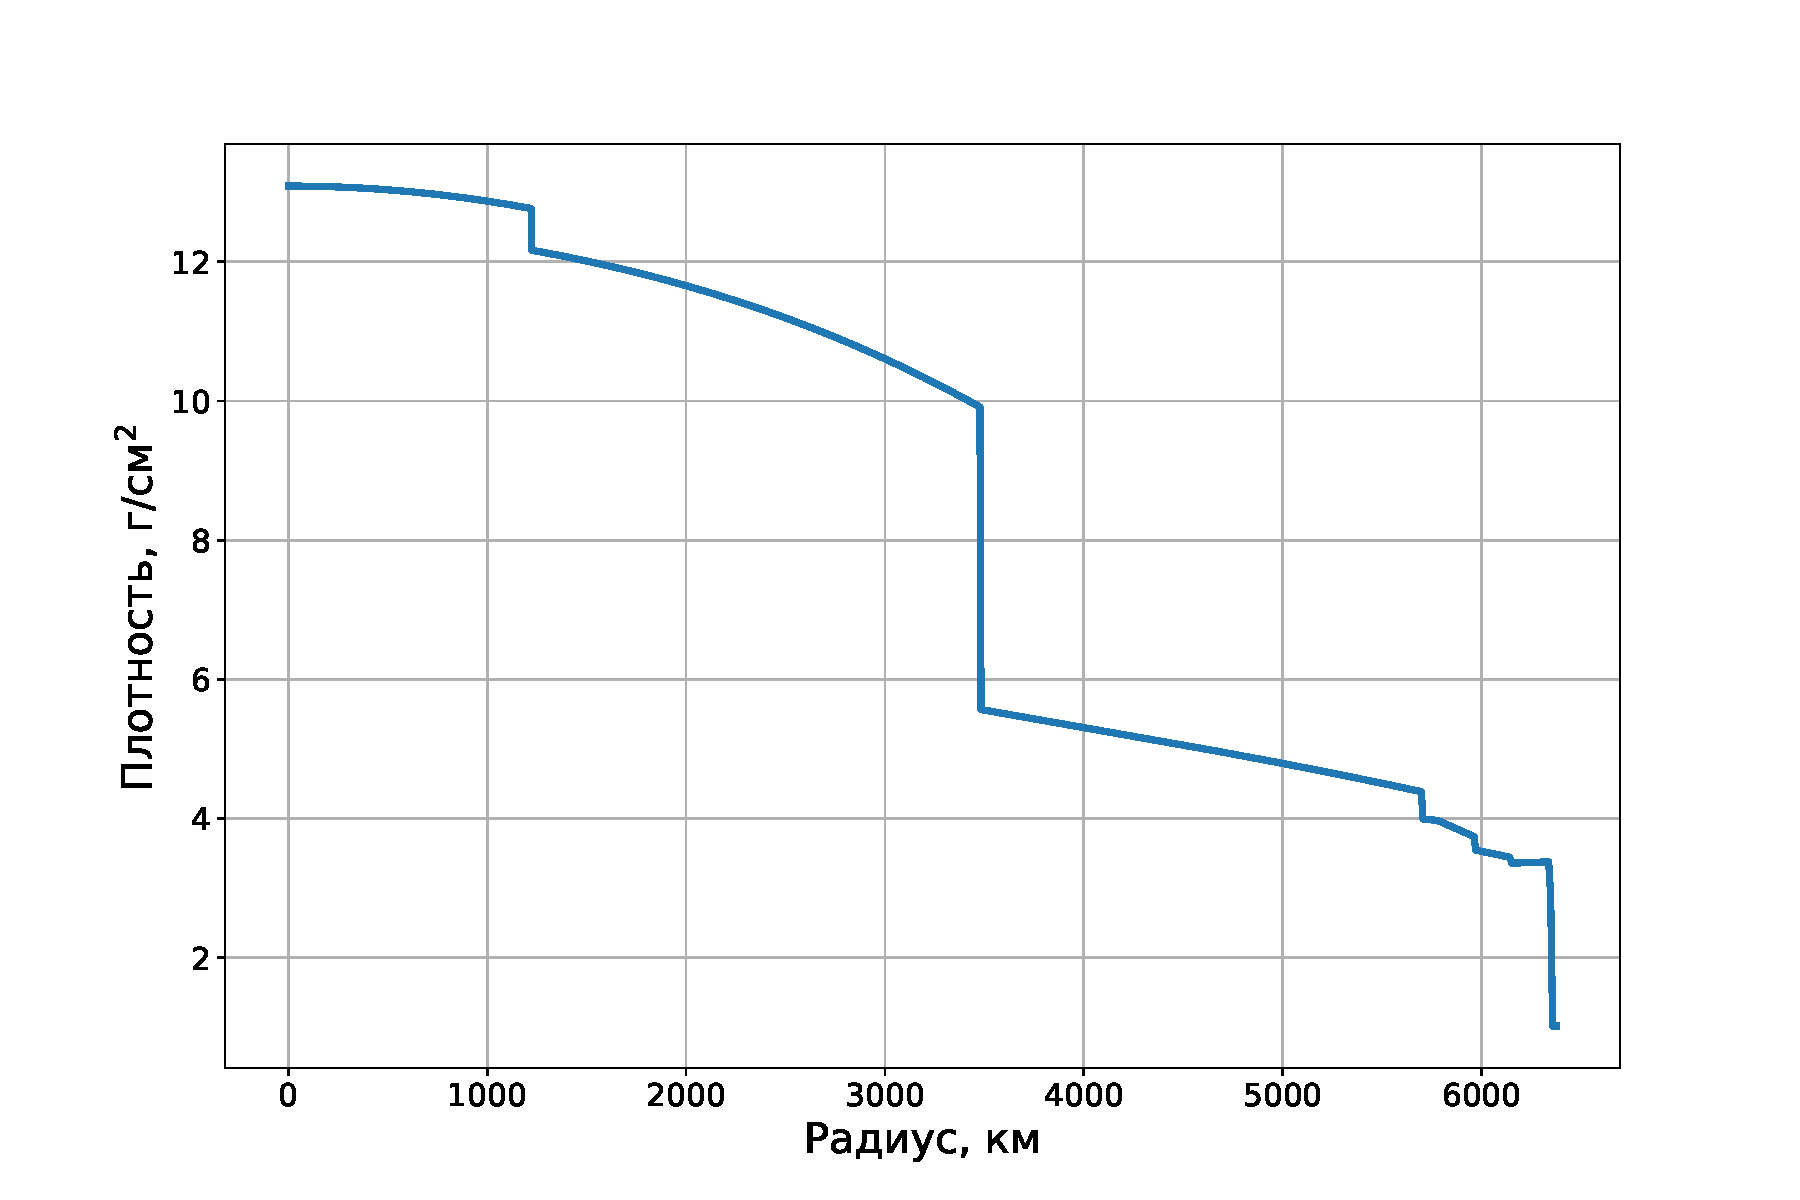
\includegraphics[width=0.8\linewidth]{images/NuProp/PREM.pdf}
\caption{Плотность вещества Земли в модели  PREM.}
\label{PREM}
\end{figure}
